\chapter{Methodologies}
\label{chapter:methodologies}
\section{Introduction to Methodologies}
At the outset of a project, it is crucial to clearly define the problem to be solved, establish the product's specification, and devise a comprehensive plan of action. This chapter outlines the design requirements and specifications for the various loudspeaker amplifier components, alongside the decisions made during the design process. These considerations are grounded in equations, simulations, and measurements. Proper execution of this step is vital, as it sets the foundation for the selection of components and ensures the effective operation of the '\emph{Booming Bass}' sound amplifier system. If this phase is not carried out correctly, it could lead to a final product that fails to meet the specified requirements of the first Integrated Project.

\section{Requirements}
\subsection{Power Supply}
The design of the power supply system for the Booming Bass Sound System is a critical step in ensuring the reliable and efficient operation of the entire sound amplifying system. The power supply is responsible for converting the AC voltage from the mains outlet, using a center-tapped transformer, into a stable DC voltage waveform. This stable DC output is essential for powering the various components of the audio system while maintaining consistent performance.

The design procedure commenced by defining and analyzing key system requirements, as well as obtaining a good understanding of the operating conditions under which the power supply needs to function. These requirements are vital for achieving the desired stability and performance. Specifically, the power supply must provide a stable DC voltage with minimal ripple under different load conditions. The target output current is 1.0 A at a voltage of $\pm$19 V at the positive and negative terminals, respectively. The voltage ripple should not exceed 5\% of its average value when under a 1.0 A load current. The ripple will be the greatest when under full load because, with a greater load, the capacitors will discharge faster, which creates a larger voltage variation between the highest and the lowest points on the waveform. To ensure safe operation, the power supply needs to discharge after use rather than leaving energy stored in the capacitors. The discharge time requirement must be met after the power supply has been left unloaded because that is when the capacitors will have the most energy stored in them.

To ensure optimal performance and reliability, several critical requirements were defined and must be met throughout the design and implementation process:

\begin{itemize}
    \item \textbf{Unloaded output voltage}: Within a $\pm$ 20-22 V DC range on the positive and negative terminal side respective.
    \item \textbf{Unloaded Operation Discharge Time}: During operation without a load, the power supply should fully discharge within a duration of 2.5 minutes. 
    \item \textbf{Load Output Voltage}: Under a load current of 1.0 A, the output voltage waveform should remain within 17-20 V DC. The power amplifier needs this voltage to amplify the audio signal without saturating adequately.
    \item \textbf{Voltage Ripple}: The voltage ripple should not exceed 5\%, in order to not distort the amplified output of the power amplifier.
    \item \textbf{Compatibility with Load Requirements}: The requirements mentioned above should still be met under a 1.0 A load, which is the design maximum load of the power amplifier.
\end{itemize}

\subsection{Power Amplifier}
The power amplifier's primary function is to amplify the voltage signal from the computer, ensuring sufficient power is delivered to the filter and ultimately to the speaker for proper operation. To meet this objective, several key requirements must be fulfilled:
\begin{enumerate}
\label{requirements PA}
    \item \textbf{Bandwidth:} The power amplifier must maintain a band-pass between 20Hz and 40kHz. 
    \item \textbf{Gain:} The amplifier is required to achieve a gain of 25 times the input signal (sound signal from the computer), corresponding to a magnitude of 27.96dB (\seautoref{eq: V to db}). 
    \item \textbf{DC Offset Management:} The DC offset must be amplified by a maximum factor of 1. 
\end{enumerate}
Requirement 1 ensures the power amplifier operates within the desired frequency range, limiting signal amplification to the specified and desired band. This approach prevents the amplification of extraneous signals, improving energy efficiency and prolonging the lifespan of circuit components.

Requirement 2 guarantees that the amplified signal is strong enough to drive the speaker effectively. This avoids signal clipping and ensures that the filer can provide adequate signal power to the loudspeaker.

Requirement 3 is critical for the preservation of the speaker's performance and signal integrity. Limiting the amplification of the DC offset by a factor of 1 prevents unnecessary noise and offset signal amplification, which could otherwise result in distortion or clipping.

\subsection{Filters}
To ensure the desired frequencies are passed to the appropriate speaker cones, filters must be carefully designed to block unwanted frequencies. This not only prevents any noise but also protects the cone from potential damage. Consequently, it is crucial to address the question: 'How can filters be effectively designed to achieve the flattest acoustic response?'.

A flat acoustic response means the filters can reproduce sound across all frequencies with minimal variation in volume. Achieving this aligns with the project's objective of delivering the highest possible sound accuracy. A flat response ensures minimal alteration in volume across frequencies, thereby enhancing sound fidelity. To meet this standard, the design process must prioritize optimal cut-off frequencies, appropriate $N$th-order filters, the decision to implement a Zobel network, and the selection of precise component values.

The filters are required to operate within a frequency range of 20Hz to 20kHz (the standard range of frequencies audible to the human ear) while maintaining maximum audio accuracy. These specifications provide significant flexibility in the design process, enabling tailored decisions to meet the project's goals and requirements.

\subsection{Loudspeaker}
A speaker functions by converting electrical current into mechanical motion, thereby generating an acoustic signal. The current passing through the voice coil induces vibrations in the speaker cone, causing a difference in sound pressure and thus producing sound waves. The speaker's physical dimensions are crucial in shaping its response to electrical inputs. To design efficient filters, it is necessary to represent the speaker's behavior with an equivalent electrical circuit. This approach facilitates precise predictions of the speaker's response to different input signals. This chapter outlines the structure of the electrical model and the methodologies used to determine its parameters.

\subsubsection{Loudspeaker Specifications}
The objective is to determine the appropriate values for the capacitors, inductors, and resistors in the electrical equivalent circuit representing the physical loudspeakers. Once these component values are identified, the circuit will be simulated over the frequency range of 20Hz to 20kHz. The simulated behavior will then be compared with the measured frequency response of the loudspeakers, ensuring that any significant deviation and discrepancy between the measured and simulated responses remains minimal to ensure high efficiency and function as projected.



\newpage
\section{Design Methodologies}
\subsection{Power Supply}
The power supply system's requirement and desired performance depend on design choices and decisions made during the project. Achieving the required performance for the Booming Bass Project necessitates careful consideration of various factors and parameters, including selecting the appropriate diodes, the values of multiple resistors, and the capacitance of smoothing capacitors. Each component mentioned must be chosen to ensure the power supply meets the specified requirements for voltage regulation, ripple percentage, and load performance. 
\begin{figure}[H]
    \centering
    \captionsetup{justification=raggedright, labelfont=bf}
    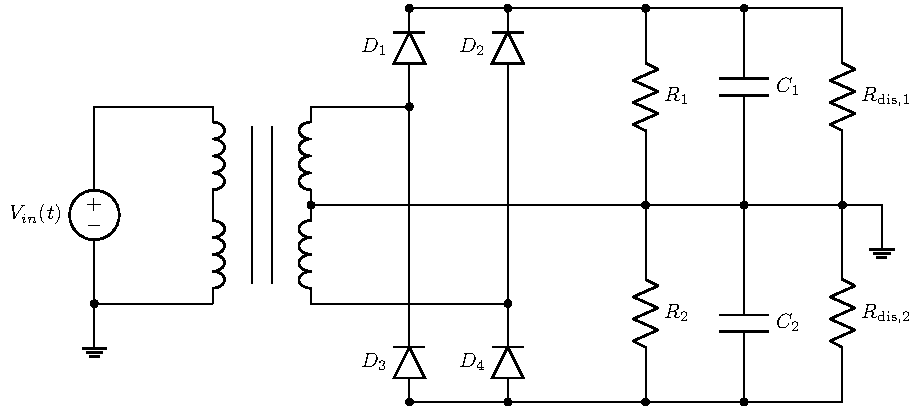
\includegraphics[width=0.75\linewidth]{TU Delft Booming Bass Project Report/figures/PowerSupply/MainPowerSupply.pdf}
    \caption{{Complete schematic of the power supply. Here, $V_{in}(t)$ represents the voltage from the wall outlet (230V, 50HZ). The primary and secondary windings are magnetically coupled, denoted by the two vertical lines indicating the magnetic core of the transformer.}}
    \label{fig:MainPowerSupplySchematic}
\end{figure}
\vspace{10pt}

The complete schematic of the power supply is shown in \sfautoref{fig:MainPowerSupplySchematic}. Each element in the schematic is clearly labeled and serves a distinct function in the design to meet the defined system requirements.
It is clear from the schematic that the power supply is dependent on multiple components and, thus, on their respective value:
\begin{itemize}
    \item \textbf{Resistors $R_{1}$ and $R_{2}$}: These resistors act and form the load of the power supply circuit, therefore simulating a real-world load. The values of the load resistors are based on the equivalent resistance of the sound-amplifying system and thus selected to ensure and to check that the output voltage remains within the desired range (e.g., 17-20 V DC) when a load current of 1.0 A is applied to the power supply circuit.
    
    \item {\textbf{Resistors} $R_{\text{dis,1}}$ \textbf{and} $R_{\text{dis,2}}$}: These resistors serve as discharge resistors, ensuring safe operation by discharging the stored energy after power supply operation. These resistors should allow the power supply to be fully discharged within 2.5 minutes after operation.
    
    \item \textbf{Capacitors $C_{1}$ and $C_{2}$}: These capacitors are essential for smoothing the rectified AC input, functioning as output filters to reduce ripple in the outgoing DC voltage at each terminal. In the power supply circuit, the AC voltage from the transformer undergoes rectification through the diodes, but fluctuations are still present in the DC output. These fluctuations are referred to as ripple. Capacitors $C_{1}$ and $C_{2}$ charge during the peaks of the DC waveform and discharge during the troughs, effectively ensuring that the DC voltage remains as stable as possible. The difference between the maximum and minimum capacitor voltage is thus called the voltage ripple. The choice of the capacitance values $C_{1}$ and $C_{2}$ and the load current determines the degree of ripple reduction and, thus, the overall stability of the output.
    
    \item \textbf{Diodes (1N5408)}: The power supply circuit diodes are responsible for rectifying the AC input into a unidirectional DC output. The actual diodes are already soldered on and differ from those chosen in the simulation process; the standard 1N4148 diodes are chosen in the LTSpice simulations for convenience.
    While they differ in primary characteristics, the 1N5408 diodes are more resilient than the 1N4148 regarding maximum repetitive peak voltage and maximum RMS voltage.
    \item \textbf{Transformer}: A center-tapped transformer to provide a dual output voltage necessary for the full wave rectification process. The transformer, therefore, provides both a positive and a negative output. The output voltage of the transformer was specified in advance and provided to the power supply subgroup.
\end{itemize}

\subsubsection{Analysis, Testing \& Measurements}
The results from simulating the circuit in LTSpice should offer valuable insight into the expected performance of the power supply, providing a theoretical understanding of its behavior.

Following the analysis of the power supply's expected performance through simulations, it is crucial to conduct real-world testing and measurements of the assembled power supply to confirm that its actual performance aligns with the predicted results. These measurements were carried out using the following:
\begin{itemize}
    \item \textbf{Oscilloscope: Tektronix TDS 2022B} An oscilloscope is necessary to conduct analysis and measurements after building the power supply to check the performance of the power supply.
    \item \textbf{Load Resistors} Large resistors are used to simulate the load of the power supply.
\end{itemize}

\subsubsection{Dimensioning Circuit Components and Elements}
Using the equation provided in the Integrated Project-1 Manual for $u_{\text{ripple}}[\%]$, the maximum voltage while maintaining a ripple percentage less than 5\% can be calculated, assuming that the average voltage after the rectifier is 19V:
\begin{flalign}\label{RippleVoltageEquation}
    u_{\text{ripple}}[\%]=\left(\frac{u_{\text{max}}-u_{\text{average}}}{u_{{average}}}\right)\cdot 100\%
\end{flalign}

Rearranging \seautoref{RippleVoltageEquation} yields the following expression for $u_{\text{max}}$:
\begin{flalign}\label{MaximumVoltageEquation}
    u_{\text{max}}=u_{\text{average}}\left(1+ \frac{u_{\text{ripple}}[\%]}{100\%}\right)
    \equnit{\si{\volt}}
\end{flalign}

Equation \ref{MaximumVoltageEquation} remains dependent on the average voltage and the ripple percentage. Therefore, the maximum voltage can be calculated for an average voltage of 19V after rectification $u_\text{average}=19V$, with $u_\text{ripple}[\%]=5\%$, which gives $u_\text{max}=19.95V$. 

\subsubsection{Smoothing Capacitors}
From the calculation, it is clear that the maximum voltage must not exceed 19.95 V to ensure that the voltage ripple remains within 5\% of the average voltage. With this constraint and limitation in place, the necessary capacitance value to keep the voltage ripple under 5\% can be determined and calculated. This calculation is based on a maximum post-rectification voltage of 19 V and during a load current of 1.0 A, using the voltage-current relationship for a capacitor:
\begin{flalign}\label{CapacitorEquation}
    I_C=C_{1,2}\frac{\mathrm{d}V_C}{\mathrm{d}t} 
    \equnit{\si{\ampere}}
\end{flalign}
For this calculation, a first-order approximation of the exponential decay of the voltage across the capacitor is applied. It is assumed that this decay follows a linear behavior, allowing it to be approximated, as shown
\begin{flalign}\label{LinearApproximation}
    \frac{\mathrm{d}V_C}{\mathrm{d}t}\approx\frac{\Delta{U_{\text{dc}}}}{\Delta{t}}
\end{flalign}
By combining Eqs. \ref{CapacitorEquation} and \ref{LinearApproximation}, the voltage-current relationship for the smoothing capacitors can be rewritten as
\begin{flalign}\label{CapacitorEquation2}
    I_C=C_{1,2}\left(\frac{\Delta U_\text{dc}}{\Delta t_{\text{dis}}}\right) 
    \equnit{\si{\ampere}}
\end{flalign}

By using \seautoref{CapacitorEquation2} and that $u_\text{max}-u_\text{average}=\frac{1}{2}\Delta U_\text{dc}$, it can be said that 
\begin{flalign}\label{CapacitanceEquation}
    C_{1,2}   &=I_C\left(\frac{1}{\left(\frac{\Delta U_{\text{dc}}}{\Delta t_\text{dis}}\right)}\right)=I\left(\frac{\Delta t_\text{dis}}{\Delta U_{\text{dc}}}\right)=I\left(\frac{\Delta t_\text{dis}}{2\left(u_{\text{max}}-u_{\text{average}}\right)}\right)
    \equnit{\si{F}}
\end{flalign}
Therefore, the required capacitance to achieve a voltage ripple below 5\% can be calculated with \seautoref{CapacitanceEquation}. Filling in for $\Delta t_\text{dis}=0.01 s$, which corresponds to half the period of 50Hz: and for the voltages $u_\text{max}=19.95V$, $u_\text{average}=19.00V$ and that $I_C=1.0A$ gives a minimum capacitance $C_{{\text{min},1,2}}=5.263$mF. 

However, it is crucial to consider that larger capacitance values could pose a significant risk due to the inrush current when the capacitor is initially charged. The rush of current occurs when the capacitor is connected to the power supply, and without sufficient series resistance, this current can spike dramatically. Larger capacitance values require more charge, leading to longer charging times and higher rush-in currents. This high current could potentially cause damage to other components if they are not rated to handle such spikes.

Additionally, larger rush-in currents can result in circuit instability, overheating of components, and thus stress on the power supply. Therefore, choosing a capacitance of $C_{{,1,2}}=6.8$mF ensures that the rush-in current remains within acceptable limits, avoiding the risks with larger capacitance values while still providing the necessary performance to meet the voltage ripple requirements. It is important to note that the calculated capacitance values apply individually to both the power supply circuit's positive and negative output terminals. Consequently, the two capacitors of equal capacitance are required to ensure proper functionality on either side of the output terminal.

\subsubsection{Discharge Resistors}\label{Discharge_Resistor_Section}
For the effective operation of the power supply and to ensure the safety of the smoothing capacitors, discharge resistors play a crucial role. Their value can be determined using the time constant of the power supply, which behaves as an RC circuit. The calculation is based on the following equation, where ${i=1,2}$ respective to each discharge resistor and each smoothing capacitor:
\begin{flalign}\label{RCCircuit}
    \tau_\text{RC}    &= R_{\text{dis,1 dis,2}}C_{1,2}
    \equnit{\si{s}}
\end{flalign}

As for the power supply circuit, the smoothing capacitors are assumed to be fully discharged after approximately 5$\tau$. Thus, it is assumed that 5$\tau\approx t_{\text{dis}}$, where $t_{\text{dis}}$ represents the discharge time. In this case, the power supply should discharge within 2.5 minutes, meaning that $t_{\text{dis,max}}=150$. Rewriting \seautoref{RCCircuit} for $R_{\text{i}}$ gives:
\begin{flalign}\label{DischargeResistor}
    R_{\text{dis,1 dis,2}}    &=\frac{\tau_\text{RC}}{C_{\text{1,2}}}=\left(\frac{{\Bigl(\frac{t_{\text{dis}}}{5}\Bigr)}}{C_{\text{1,2}}}\right)=\frac{t_{\text{dis}}}{5C_{\text{1,2}}}
    \equnit{\si{\Omega}}
\end{flalign}

Using formula \ref{DischargeResistor}, the previously calculated capacitance, $t_\text{dis}=105 s$ gives a discharge resistor of 5.7k$\Omega$. A discharge resistance of 5.7k$\Omega$ for $R_\text{dis,1}$ and $R_\text{dis,2}$ respectively ensures that the power supply fully discharges within 2.5 minutes, given a smoothing capacitance of 5.263mF at each side of the output terminals. The calculations and the corresponding \seautoref{DischargeResistor} show that reducing the discharge resistance will result in a shorter discharge time for the power supply.

The sizing of the discharge resistor influences the ripple voltage, though in some cases, its effect may be negligible. Ripple voltage arises from fluctuations in voltage as the smoothing capacitor $C_{s1,s2}$ charges and discharges between full-wave rectified peaks. The discharge resistor $R_{\text{dis}1,\text{dis}2}$ affects the discharge rate, thus influencing the ripple's extent. Higher discharge resistor values cause the smoothing capacitors to discharge more slowly, maintaining a higher voltage for a longer period between rectified peaks, resulting in a smaller ripple. With less current drawn by the load, the capacitor discharges more gradually. Conversely, lower discharge resistor values cause faster discharge, leading to a larger ripple as the voltage drops more quickly between peaks.

In some designs, the effect of the discharge resistor can be negligible if its resistance is high compared to the capacitance. In such cases, the capacitor discharges slowly, resulting in a small ripple. Therefore, the impact of the discharge resistor on the ripple may be minimal in these scenarios.

\subsection{Power Amplifier}
\label{section: design PA}

\subsubsection{Power Amplifier Circuit}
To construct the amplifier circuit, a universal power amplifier was utilized (see \sfautoref{fig: universal power-amp}). This circuit includes several components without predefined values. To determine these values, the amplifier was first divided into three distinct sections for simplification:
\begin{itemize}
    \item A passive Low-Pass Filter (p-LPF)
    \item A passive High-Pass Filter (p-HPF)
    \item An active High-Pass Filter (a-HPF)
\end{itemize}

All of these filters are first-order systems because they use a single capacitor, and their corresponding transfer functions are first-order expressions. (refer to \seautoref{eq: E}, \seautoref{eq: F} and \seautoref{eq: G}).

To ensure optimal performance of the power amplifier, the cut-off frequencies of these three filters must be spaced by a factor of 10. This separation minimizes the risk of interference between the filters and guarantees their proper functionality. The calculations of the required component values will be based on the application of the following fundamental formulas, which are detailed in this section:
\begin{flalign}
    \label{eq: V to db}
    \mathbf{H(\omega)} = 20\log\left(\frac{V_o}{V_i}\right)
    \equnit{\si{dB}}
\end{flalign}

where $V_o$ and $V_i$ are the output and input voltages, respectively. This equation allows the gain to be expressed on a dB scale. The expected gain for a non-inverting amplifier circuit is calculated as:
\begin{flalign}
    \label{eq: noninvert}
    \mathbf{G}_{\text{gain}}=\frac{V_o}{V_i}= \frac{R_f}{R_i}+1
\end{flalign}

where $R_f$ and $R_i$ are the feedback and input resistances, respectively. This equation is used to determine the amplification factor of the non-inverting amplifier circuit. To calculate the phase shift at a given frequency in the transfer function, the following equation is used:
\begin{flalign}
    \label{eq: phase}
    \phi = \arctan{\frac{\mathbf{X_{H(\omega)}}}{\mathbf{R_{H(\omega)}}}}, \qquad \mathbf{H(\omega)} = R+jX
\end{flalign}

Here, $\mathbf{X_{H({\omega})}}$ and $\mathbf{R_{H({\omega})}}$ are the imaginary and real components of the impedance, respectively. This allows the determination of the phase shift at a given frequency, which is crucial for understanding the behavior of the amplifier circuit in terms of signal timing.
Other relevant formulas will be introduced and derived in their respective sections as needed.

\subsubsection{Calculations with one circuit design}
In the course of this project, two power amplifiers were constructed- one by group B2-1 and another by group B2-2. To determine which amplifier would be integrated into the final loudspeaker system, both circuits were evaluated against the three key requirements outlined in \autoref{requirements PA} (Refer to \autoref{section: choosing a circuit} to see the evaluation). The chosen circuit is B2-1's power amplifier. For this reason, only the exact calculations for this amplifier will be shown. However, to derive the values of B2-2's amplifier, the same methods were used, only other base values were chosen.


\subsubsection{Passive High-Pass Filter (p-HPF)}
The circuit diagram of a passive high-pass filter used in the power amplifier circuit is shown in \ref{fig: pa high pass}.
\begin{figure}[H]
    \centering
    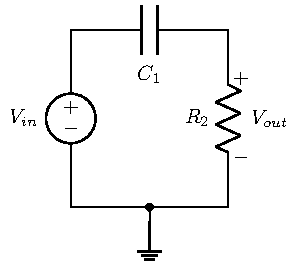
\includegraphics[width=0.3\linewidth]{TU Delft Booming Bass Project Report/figures/PowerAmplifier/circuits/HighPass filter.pdf}
    \captionsetup{justification=raggedright, labelfont=bf}
    \caption{The circuit of a passive high-pass filter.}
    \label{fig: pa high pass}
\end{figure}

The transfer function of this p-HPF circuit is derived by applying a voltage divider approach to the circuit. Initially, the conditions hold that $\mathbf{V_{out}=V_o}$:
\begin{flalign}
    \mathbf{V_o} &= \mathbf{V_i}\frac{Z_{R_2}}{Z_{R_2}+Z_{C_1}}
    \equnit{\si{V}}
\end{flalign}

This leads to the following expression for the voltage gain:
\begin{flalign}
    \mathbf{\frac{V_o}{V_i}}    &= \frac{Z_{R_2}}{Z_{R_2}+Z_{C_1}}= \frac{R_2}{R_2 + \frac{1}{sC_1}}
\end{flalign}

where $s=j\omega$. Simplifying this further and rearranging terms, the transfer function for the given p-HPF circuit is:
\begin{flalign}
\label{eq: E}
    \mathbf{E(\omega)}=\mathbf{\frac{V_o}{V_i}} = \frac{sC_1R_2}{sC_1R_2 +1 }
\end{flalign}

This transfer function confirms that the circuit behaves as a passive high-pass filter (p-HPF), as the following limits hold true for a typical RC high-pass filter circuit:
\begin{flalign}
    \lim_{\omega \rightarrow 0}\mathbf{E(\omega)}= 0\\
    \lim_{\omega \rightarrow \infty}\mathbf{E(\omega)}=1
\end{flalign}

These results are consistent with the characteristics of a high-pass filter. To determine the values of $R_a$ and $C_a$, the cut-off frequency can be derived as a function of these components. This derivation can be done by using the transfer function:
\begin{flalign}
    \mathbf{E(\omega)} = \mathbf{\frac{V_o}{V_i}} = \frac{sC_{1}R_{2}}{sC_{1}R_{2} + 1} = \frac{s}{\omega_0}\left(\frac{1}{1 + \frac{s}{\omega_0}}\right) 
\end{flalign}

Where and:
\begin{flalign}\label{eq: cutoff high}
    \omega_0 = \frac{1}{R_{2}C_{1}}
    \equnit{\si{\text{rad s^{-1}}}}
\end{flalign}

Given that $R_2=47\text{k}\Omega$ is predetermined and the desired cut-off frequency is 20Hz, the value of $C_1$ can be calculated as follows:
\begin{flalign}
    C_1 = \frac{1}{40\pi(47\cdot10^3)} = 169.3\text{nF}
    \equnit{\si{nF}}
\end{flalign}

Thus, to achieve a cut-off frequency for the passive high-pass filter of 20Hz with $R_2=47\text{k}\Omega$, the required value for $C_1$ is 169.3nF.

\subsubsection{Passive Low-Pass Filter (p-LPF)}
The circuit diagram of a passive low-pass filter used in the power amplifier circuit is shown in \sfautoref{fig: pa low pass}:
\begin{figure}[h]
    \centering
    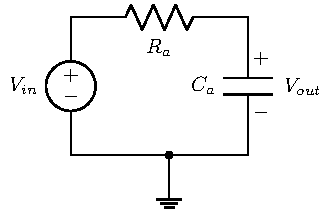
\includegraphics[width=0.3\linewidth]{TU Delft Booming Bass Project Report/figures/PowerAmplifier/circuits/LowPass filter.pdf}
    \captionsetup{justification=raggedright, labelfont=bf}
    \caption{The circuit of a passive low-pass filter .}
    \label{fig: pa low pass}
\end{figure}

The transfer function of this p-LPF circuit is derived by applying the same voltage divider approach to the circuit as with the p-HPF circuit. Initially, the conditions hold that $\mathbf{V_{out}=V_o}$:
\begin{flalign}
    \mathbf{V_o} = \mathbf{V_i}\frac{Z_{C_a}}{ Z_{R_a}+Z_{C_a}}
    \equnit{\si{V}}
\end{flalign}

This leads to the following expression for the voltage gain:
\begin{flalign}
    \mathbf{\frac{V_o}{V_i}} = \frac{Z_{C_a}}{ Z_{R_a}+Z_{C_a}}= \frac{\frac{1}{sC_a}}{R_a + \frac{1}{sC_a}}
\end{flalign}

where $s=j\omega$. Simplifying this further and rearranging terms, the transfer function for the given p-LPF circuit is:
\begin{flalign}\label{eq: F}
    \mathbf{F(\omega)} = \mathbf{\frac{V_o}{V_i}} = \frac{1}{sC_aR_a +1}
\end{flalign}

This transfer function confirms that the circuit behaves as a passive low-pass filter (p-LPF), as the following limits hold true for a typical RC low-pass filter circuit:
\begin{flalign}
    \lim_{\omega \rightarrow 0}\mathbf{F(\omega)}= 1\\
    \lim_{\omega \rightarrow \infty}\mathbf{F(\omega)}=0
\end{flalign}

These results are consistent with the characteristics of a low-pass filter. To determine the values of $R_a$ and $C_a$, the cut-off frequency can be derived as a function of these components. This derivation can be done by using \seautoref{eq: F}, thus giving us a similar transfer function as \seautoref{eq: cutoff high}:
\begin{flalign}
    \mathbf{F(\omega)} = \frac{1}{sC_{a}R_{a}+1} = \frac{1}{\left(\frac{s}{\omega_0} + 1\right)}
\end{flalign}

where $s=j\omega$, and: 
\begin{flalign}\label{eq: cutoff low}
    \omega_0 = \frac{1}{R_{a}C_{a}}
    \equnit{\si{\text{rad s^{-1}}}}
\end{flalign}

The value of $R_a$ was selected as 1k$\Omega$ due to its simplicity for calculations. Given a cut-off frequency of 40kHz for the p-LPF, and $R_a=1\text{k}\Omega$, the corresponding value for $C_a$ is calculates as:
\begin{flalign}
    C_a = \frac{1}{80\text{k}\pi\left(1.0\cdot 10^{3}\right)} = 3.98\text{nF}
    \equnit{\si{nF}}
\end{flalign}

Thus, to achieve a cut-off frequency for the passive low-pass filter (p-LPF) of 40kHz with $R_a=1\text{k}\Omega$, the required value for $C_a$ is 3.98nF.


\subsubsection{Active High-Pass Filter (a-HPF)}
The circuit diagram of an active high-pass filter is shown in \sfautoref{fig: pa active high pass}:
\begin{figure}[H]
    \centering
    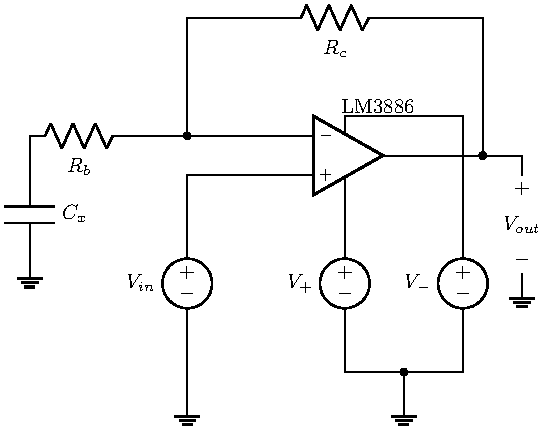
\includegraphics[width=0.4\linewidth]{TU Delft Booming Bass Project Report/figures/PowerAmplifier/circuits/active_high_pass.pdf}
    \captionsetup{justification=raggedright, labelfont=bf}
    \caption{The circuit of an active high-pass filter (a-HPF).}
    \label{fig: pa active high pass}
\end{figure}

The final filter is an active high-pass filter. In this filter, $C_x$ serves a crucial role in blocking any DC voltage from reaching the operational amplifier (op-amp). This DC voltage could originate from the input signal or from an offset voltage between the two input terminals of the op-amp, which results from its non-ideal characteristics. By blocking the DC component, this function prevents any residual DC voltage from being amplified, thus protecting the loudspeaker from potential damage.

As specified in the IP-1 manual \cite{IP-manual}, the op-amp used in this power amplifier circuit is the 'LM3886 Operational Amplifier'. The LM3886 offers several beneficial properties, mentioned in \cite{IP-manual}:

\begin{enumerate}
    \item A high input resistance of 200k$\Omega$. 
    \item A low output resistance of 10$\Omega$. 
    \item A large open-loop voltage gain of $10^5$.
\end{enumerate}

These characteristics are relatively close to ideal, allowing calculations involving the LM3886 to be made under the assumption that it behaves as an ideal op-amp.

The transfer function for this active high-pass filter can be derived using nodal analysis at the input terminals of the op-amp:
\begin{flalign}
    \mathbf{V_{in} = V_{-}}
    \equnit{\si{V}}
\end{flalign}
where the input voltage $V_{in}$ equals the negative op-amp voltage, denoted by $V_{-}$. Nodal analysis on the active high-pass filter circuit gives:
\begin{flalign}
    \frac{V_i}{Z_{R_b}+Z_{C_x}} = \frac{V_{o}-V_{i}}{Z_{R_c}}\\
    \left(\frac{1}{R_b + Z_{C_x}} + \frac{1}{R_C}\right)V_i = \frac{V_o}{R_c}
\end{flalign}

Simplifying this further and rearranging terms, the transfer function for the given a-HPF circuit is:
\begin{flalign}
    \label{eq: G}
    \mathbf{G(\omega)} = \mathbf{\frac{V_o}{V_i}} = \frac{R_C}{R_b + \frac{1}{s C_x}}+1
\end{flalign}

The behavior of an a-HPF can again be shown by $\omega$ approaching 0 and $\infty$:

\begin{flalign}
    \lim_{\omega \rightarrow 0}\mathbf{G(\omega)}= 1\\
    \lim_{\omega \rightarrow \infty}\mathbf{G(\omega)}=\frac{R_c}{R_b} + 1
\end{flalign}

At very low frequencies, the gain goes to 1, while at very high frequencies, $C_x$ acts as a short circuit, allowing the a-HPF filter to achieve its maximum gain. This behavior is characteristic to an active high-pass filter. 


Since this circuit also functions as a high-pass filter, \seautoref{eq: cutoff high} can be applied again, substituting $R_2$ and $C_1$ with $R_b$ and $C_x$ respectively to calculate the relevant values. The role of $C_x$ is to prevent amplification of the DC offset generated within the op-amp. As the frequency approaches zero, the impedance of $C_x$ increases, causing it to behave like an open circuit and turning the amplifier into a voltage follower. Given that this frequency must be an order of 10 lower than the low-pass filter cut-off frequency, a frequency of 2Hz was selected. Using $R_b=80\text{k}\Omega$ (chosen for the ease of obtaining a simple value for $C_x$) and $f=2\text{Hz}$, the value of $C_x$ can be calculated as follows: 
\begin{flalign}
    C_x = \frac{1}{4\pi(80\cdot10^{3})} = 1 \mathrm{\mu F}
    \equnit{\si{\mu{F}}}
\end{flalign}


\subsubsection{Calculating $\mathbf{R_c}$}

To calculate $R_c$, capacitor $C_x$ can be considered a short circuit, as the cut-off frequency is 2Hz, which is a decade lower than the frequencies expected to pass through the circuit. In this scenario, the circuit behaves as a standard non-inverting amplifier. Therefore, \seautoref{eq: noninvert} can be applied, where $R_f$ and $R_i$ correspond to $R_c$ and $R_b$, respectively, assuming the op-amp operates ideally. Using $R_b=80\text{k}\Omega$ and a voltage gain of $\mathbf{V_o}$/$\mathbf{Vi}$=25, the value of $R_c$ can be determined as follows:

\begin{flalign}
   \frac{V_o}{V_i}  &= \frac{R_c}{R_b}+ 1 \Rightarrow R_c=R_b(25-1)=24R_b\\
    R_c &=1.92\text{M}\Omega
\end{flalign}

To verify this ratio, nodal analysis was performed on the active high-pass filter circuit, assuming non-ideal conditions. For simplification, a resistor value of 1k$\Omega$ was used for $R_b$ instead of 80k$\Omega$, which aided in streamlining the subsequent calculations (refer to \autoref{calculation of Rc} for the complete calculation). 

To further validate that the entire power amplifier circuit operates as a band-pass filter, the transfer function of the full circuit was derived. The transfer function in  \seautoref{eq: E}, \seautoref{eq: F}, and \seautoref{eq: G} were multiplied together to obtain the total transfer function (see \autoref{total transfer} for the complete calculation and derivation). The resulting response is as follows:

% Just to confirm that the complete power amplifier circuit behaves as a band-pass filter (BPF), this is again done with a transfer function. To obtain the complete transfer function of the circuit,  \seautoref{eq: E}, \seautoref{eq: F}, and \seautoref{eq: G} have to be multiplied by each other (for the full calculation, see \autoref{total transfer}). This response ended up being:  
\begin{flalign}\label{eq: total transfer}
    \mathbf{H(\omega)} = \frac{s^2 (af+ k) + s a }{e \big(sf + 1 \big)}
\end{flalign}

where $a=R_{2}C_{1}$, $b=R_{a}C_{a}$, $d=ab$, $f=R_{b}C_{x}$, $k=aR_{c}C_{x}$, and $e=s^{2}d+sa+sb+1$.
This transfer function confirms the band-pass nature of the circuit, as the following limits hold true:
\begin{flalign}
    \lim_{\omega \rightarrow 0}\mathbf{H(\omega)}= 0\\
    \lim_{\omega \rightarrow \infty}\mathbf{H(\omega)}=0
\end{flalign}

This behavior of the transfer function $\mathbf{H(\omega)}=0$ is immediately apparent when $\omega$ goes to infinity and can be explained by the structure of the transfer function; the numerator is a second-order equation, while the denominator is a third-order equation. As $\omega$ approaches infinity, the denominator increases at a faster rate than the numerator, causing the entire equation to approach zero (see \seautoref{eq: third order}).

\begin{figure}[H]
    \centering
    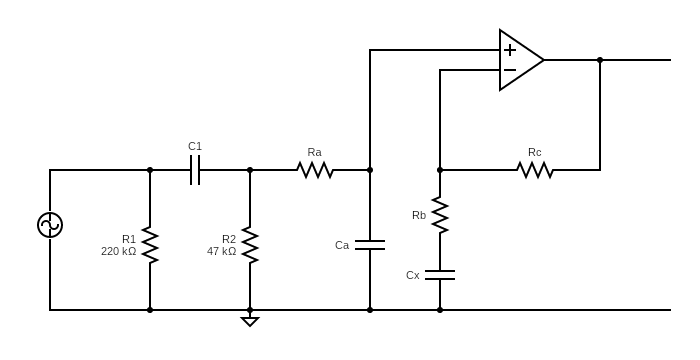
\includegraphics[width=0.7\linewidth]{TU Delft Booming Bass Project Report/figures/PowerAmplifier/circuits/circuit.png}
    \captionsetup{justification=raggedright, labelfont=bf}
    \caption{A universal circuit for a power amplifier.}
    \label{fig: universal power-amp}
\end{figure}

In the lab, components are not available at every possible value. As a result, the ideal values calculated for the power amplifier circuit could not be directly implemented; instead, they were replaced with components whose values were as close as possible to the initially calculated values. The calculated ideal values and the final chosen values are listed in \stautoref{tab:B2-1 ideal values}. Since the power amplifier used in the final system is from group B2-1, all calculations in this section are based on the data from B2-1's power amplifier. Data obtained by group B2-2 are presented in \stautoref{tab:B2-1 ideal values}.


\begin{table}[H]
    \centering
    \caption{B2 Summary of calculated and chosen (Resistance $R_N$, capacitance $C_N$, and cut-off frequency $f_{\text{cut-off}}$) values for the p-HPF, p-LPF, a-HPF, with $D_{\text{diff}}[\%]$ representing the deviation between the calculated and used values.}
    \resizebox{\textwidth}{!}{
    \begin{tabular}{c @{\hspace{12pt}} *4{c} S @{\hspace{12pt}} *4{c} S @{\hspace{12pt}}}
        \toprule
        \multicolumn{9}{c}{\textbf{B2 Filter Component Parameters}} \\
        \cmidrule(lr){1-9}
        & & \multicolumn{3}{c}{\textbf{B2-1 Component Values}} & & \multicolumn{3}{c}{\textbf{B2-2 Component Values}} \\
        \cmidrule(lr){3-5} \cmidrule(lr){7-9}
        & Parameter & Calc. Value & Used Value & $D_{\text{diff}}$ [\%] & & Calc. Value & Used Value & $D_{\text{diff}}$ [\%] \\
        \midrule
        p-HPF & $R_2$ [$\Omega$] & 47k$\Omega$ & 47k$\Omega$ & 0.00\% & & 47k$\Omega$ & 47k$\Omega$ & 0.00\% \\
         & $C_1$ [F] & 169.3nF & 166.5nF & -1.65\% & & 169.3nF & 220nF & 29.94\% \vspace{4pt} \\
         & $f_\text{cut-off}$ [Hz] & 20Hz & 20Hz & 0.00\% & & 13Hz & 20Hz & 53.85\% \vspace{10pt} \\
        p-LPF & $R_a$ [$\Omega$] & 1k$\Omega$ & 987$\Omega$ & -1.3\% & & 12$\Omega$ & 680$\Omega$ & 5567\% \\
         & $C_a$ [F] & 3.98nF & 4.05nF & -1.73\% & & 330nF & 6.8nF & -97.96\% \vspace{4pt}\\
         & $f_\text{cut-off}$ [Hz] & 40kHz & 40kHz & 0.00\% & & +100kHz & 34kHz & - \vspace{10pt}\\
        a-HPF & $R_c$ [$\Omega$] & 1.92M$\Omega$ & 1.92M$\Omega$ & 0.00\% & & 1.92M$\Omega$ & 1.92M$\Omega$ & 0.00\% \\
        & $R_b$ [$\Omega$] & 80k$\Omega$ & 81.8k$\Omega$ & 2.25\% & & 2kM$\Omega$ & 2k$\Omega$ & 0.00\% \\
         & $C_x$ [F] & 1$\mu$F & 968nF & -1.4\% & & 8.3$\mu$F & 8.2$\mu$F & -1.20\% \vspace{4pt} \\
         & $f_\text{cut-off}$ [Hz] & 2Hz & 2Hz & 0.00\% & & 9.6Hz & 9.6Hz & 0.00\% \\
        \bottomrule
    \end{tabular}
    }
    \captionsetup{justification=raggedright, labelfont=bf}
    
    \label{tab:B2-1 ideal values}
\end{table}

\subsection{Filters - Loudspeaker Circuit Models}
\subsubsection{Model at Resonant Frequency}
The behavior of the speakers can be represented by an equivalent circuit comprising resistors, capacitors, and inductors. The capacitors and inductors model the speaker's frequency-dependent characteristics. At certain frequencies, the speaker exhibits predominantly higher resistive behavior, primarily influenced by the natural resonant frequency of the speaker's cone. The circuit model consists of five elements arranged as shown in \sfautoref{fig:impedance_model1}. Here, $R_e$ represents the impedance at DC conditions, $L_e$ models the inductance of the voice coil, and the parallel RLC branch represents the mechanical properties of the cone. In this parallel branch, $R_p$ corresponds to frictional losses, $L_p$ models the mass of the cone, and $C_p$ represents its spring-like behavior \cite{johnshopkins_rlc}.
\begin{figure}[H]
    \centering
    \captionsetup{justification=raggedright, labelfont=bf}
    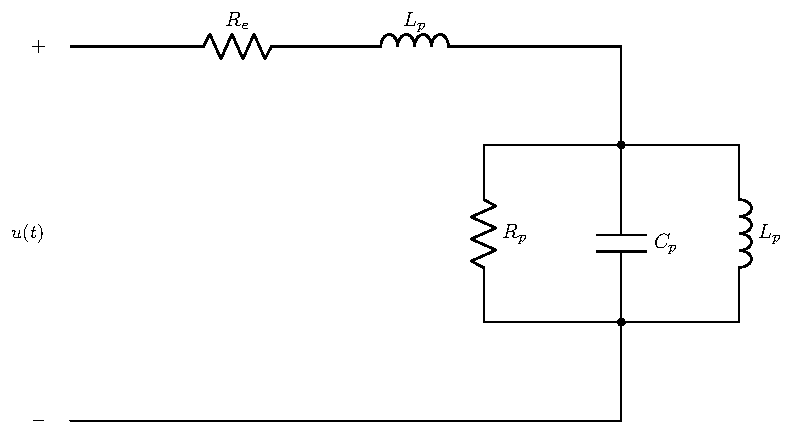
\includegraphics[width=0.6\linewidth]{figures/FilterGroup/ImpedanceModel1.pdf}
    \caption{Impedance model of the loudspeakers, depicting the equivalent circuit configuration used to represent the speaker's electrical ($R_e$, $L_e$) and mechanical properties ($R_p$, $C_p$, $L_p$ )\cite{IP-manual}.}
    \label{fig:impedance_model1}  
\end{figure}

\subsubsection{Model above Resonant Frequency}
At frequencies above and significantly higher than the cone's resonant frequency, the equivalent circuit can be further simplified. The total impedance of the circuit could be calculated using \seautoref{eq:total impedance}. For $\omega \gg \omega_o$, where $\omega_o$ is the resonant frequency of the circuit, the parallel components $R_p, C_p$ and $L_p$ can be disregarded due to their diminished influence on the overall impedance. To justify this simplification, the analysis should employ a normalized angular frequency $\omega'$ defined as follows:
\begin{flalign}
    \label{eq:normalize frequency}
    \omega' = \frac{\omega}{\omega_o}
%    \equnit{\si{\text{rad s^{-1}}}}  Heeft geen units, want normalized
\end{flalign}
The total impedance of the loudspeaker model is given by
\begin{flalign}
    \label{eq:total impedance}
    Z_{tot} = R_e + j\omega L_e + \frac{1}{\frac{1}{R_p}+j\omega C_p+\frac{1}{j\omega L_p}}
    \equnit{\si{\Omega}}
\end{flalign}

By applying \seautoref{eq:normalize frequency} and substituting it into \seautoref{eq:total impedance}, a revised expression for the total impedance, $Z_{tot}$, is obtained, as presented in \seautoref{eq:normalized impedance}:
\begin{equation}
    \label{eq:normalized impedance}
    Z_{tot} = R_e + j\frac{\omega'}{\sqrt{L_pC_p}}L_e + \frac{1}{\frac{1}{R_p}+j\sqrt{\frac{C_p}{L_p}}\left(\omega'-\frac{1}{\omega'}\right)}
    \equnit{\si{\Omega}}
\end{equation}

The angular frequency $\omega$ can be expressed as $\omega'\omega_o$, where $\omega'$ is the normalized angular frequency, and $\omega_o$ is the resonant frequency. Substituting the expression for $\omega_o$ from Eq.\ref{eq:resonant frequency appA}\cite{IP-manual}, the final expression for $\omega$ is derived and presented in \seautoref{eq:final omega appA}.
\begin{flalign}
    \label{eq:resonant frequency appA}
    \omega_o = \frac{1}{\sqrt{L_pC_p}}
    \equnit{\si{\text{rad s^{-1}}}}
\end{flalign}
\begin{flalign}
    \label{eq:final omega appA}
    \omega = \frac{\omega'}{\sqrt{L_pC_p}}
    \equnit{\si{\text{rad s^{-1}}}}
\end{flalign}

In the following section, $Z_{par}$ will be defined as the impedance of the parallel RLC portion of the equivalent circuit. Its expression is provided in \seautoref{eq:parallel impedance appA}:
\begin{flalign}
    \label{eq:parallel impedance appA}
    Z_{par} = \frac{1}{\frac{1}{R_p}+j\omega C_p+\frac{1}{j\omega L_p}}
    \equnit{\si{\Omega}}
\end{flalign}


To examine the behavior of $Z_{par}$ when $\omega \gg \omega_o$, we can investigate the impedance as $\omega'\gg 1$. To do this first, we first need to rewrite the equation in terms of $\omega'$:
\begin{flalign}
\label{eq:capacitive_impedance appA}
    j\omega C_p = j\omega'\sqrt{\frac{c_p}{L_p}}
    \equnit{\si{\Omega^{-1}}}
\end{flalign}

\begin{flalign}
\label{eq:inductive_impedance appA}
    \frac{1}{j\omega L_p} = -j\frac{1}{\omega'}\sqrt{\frac{C_p}{L_p}}
    \equnit{\si{\Omega^{-1}}}
\end{flalign}

Substituting Eq~\ref{eq:capacitive_impedance appA} and Eq~\ref{eq:inductive_impedance appA} into Eq~\ref{eq:parallel impedance appA} will result in Eq~\ref{eq:normalized impedance appA}.

\begin{flalign}
    \label{eq:normalized impedance appA}
    Z_{par} = \frac{1}{\frac{1}{R_p}+j\sqrt{\frac{C_p}{L_p}}(\omega'-\frac{1}{\omega'})}
    \equnit{\si{\Omega}}
\end{flalign}

It can now be observed that if $\omega'\gg1$, then $Z_{par} \ll 1$. Since $Z_{tot} = R_e + j\omega L_p + Z_{par}$, it follows that for $\omega \gg \omega_o$, the total impedance can be approximated as $Z_{tot} \approx R_e + j\omega L_p$.

The revised expression for $Z_{tot}$ corresponds to an equivalent circuit consisting of an inductor and a resistor, as shown in Fig \ref{fig:impedance_model2}. If the operating frequencies of the speaker are all significantly higher than the resonant frequency, utilizing this simplified model becomes more practical for analysis and design purposes.
\begin{figure}[H]
    \centering
    \captionsetup{justification=raggedright, labelfont=bf}
    \includegraphics[width=0.5\linewidth]{figures/FilterGroup/impedance_model2_speaker.jpg}
    \caption{Impedance model for frequencies above the resonant frequency, illustrating the simplified equivalent circuit consisting of an inductor $L_e$ and the resistor $R_e$ \cite{IP-manual}.}
    \label{fig:impedance_model2}
\end{figure}

\subsubsection{Calculate Model Parameters}
The determination of the five unknown parameters requires solving a set of five equations. By analyzing the circuit and its impedance, the necessary equations for parameter estimation can be derived. The measured impedance data is presented in Fig \ref{fig:abs_speakers}. Detailed derivations of these equations are provided in the IP-manual \cite{IP-manual}.
\begin{flalign}
    \label{eq:Re_model}
    R_e = \left. |Z| \right._{\omega=0}
    \equnit{\si{\Omega}}
\end{flalign}

Where $R_e$ represents the equivalent resistance of the circuit under DC conditions, corresponding to the impedance when the frequency is zero ($\omega=0$). Similarly, the parallel resistance $R_p$ is derived by subtracting $R_e$ from the magnitude of the total impedance $|Z|$ at the resonant angular frequency denoted by $\omega= \omega_o$, as given in \seautoref{eq:Rp_model}:
\begin{flalign}
    \label{eq:Rp_model}
    R_p = \left. |Z| \right._{\omega=\omega_o} - R_e
    \equnit{\si{\Omega}}
\end{flalign}

Where $R_p$ accounts for the frictional losses in the mechanical behavior of the speaker at resonance. The capacitance $C_p$, representing the spring behavior of the speaker cone, is related to $R_p$ by \seautoref{eq:Cp_model}:
\begin{flalign}
    \label{eq:Cp_model}
    C_p = \frac{1}{R_pB}
    \equnit{\si{F}}
\end{flalign}

Where B characterizes the bandwidth of the speaker's cone, the inductance $L_p$, representing the mass of the speaker cone, is related to $C_p$ and the resonant angular frequency $\omega_o$ by \seautoref{eq:Cp_model}. 
The inductance $L_e$, which models the voice coil, can be derived from the impedance at high frequencies ($\omega \gg \omega_o$) using Eq \ref{eq:Le_model}:
\begin{flalign}
    \label{eq:Lp_model}
    L_p = \frac{1}{C_p\omega_o^2}
    \equnit{\si{H}}
\end{flalign}
\begin{flalign}
    \label{eq:Le_model}
    L_e = \frac{\sqrt{(|Z|_{\omega \gg \omega_o})^2-R_e^2}}{\omega}
    \equnit{\si{H}}
\end{flalign}

The next step involves solving the equations for the different speakers and simulating the models to compare their responses with the actual measured data. Tab.\ref{tab:speaker_components} presents the calculated component values.
\begin{figure}[H]
    \centering
    \begin{minipage}{0.5\textwidth}
        \centering
        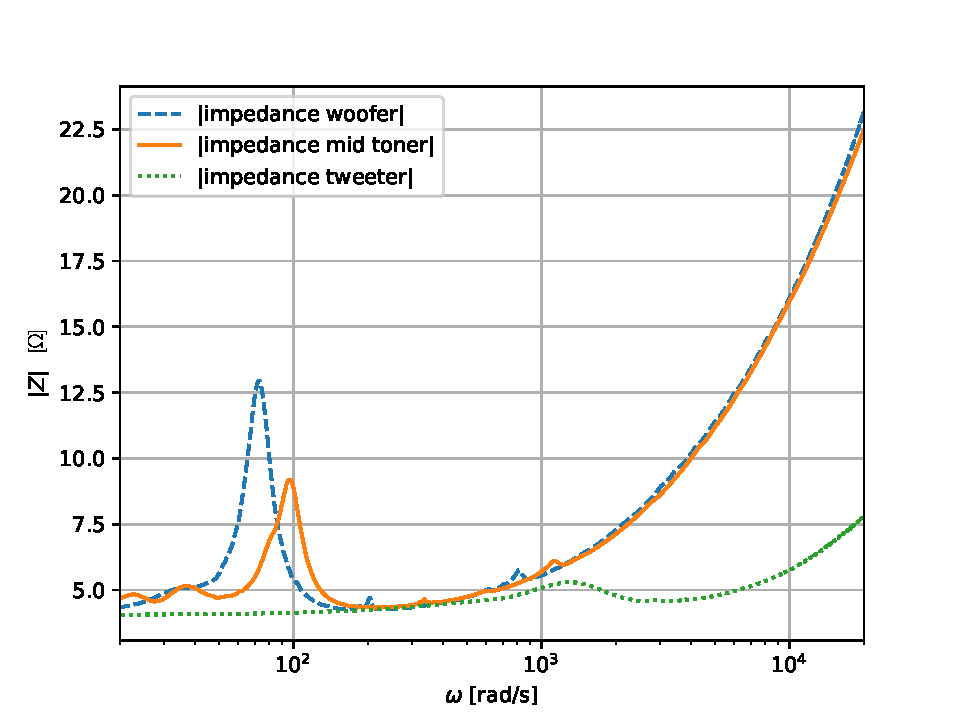
\includegraphics[width=\linewidth]{TU Delft Booming Bass Project Report/figures/FilterGroup/abs_impedance_speakers (2).pdf}
        \captionsetup{justification=raggedright, labelfont=bf}
        \caption{Absolute value of the speaker impedance.}
        \label{fig:abs_speakers}
    \end{minipage}\hfill
    \begin{minipage}{0.5\textwidth}
        \centering
        \captionsetup{justification=raggedright, labelfont=bf}
        \caption{Component Values for the woofer, tweeter, and mid-toner, showing each component's resistance, inductance, and capacitance values. The table highlights the different characteristics of the components used in the speaker system.}
        \begin{threeparttable}
          \centering
          \begin{tabular}{c @{\hspace{12pt}} *4{c} S @{\hspace{12pt}}}
            \toprule
            \multicolumn{5}{c}{\textbf{Speaker Component Values}} \\
            \cmidrule(lr){1-5}
            & & \multicolumn{3}{c}{\textbf{Component Values}} \\
            \cmidrule(lr){3-5}
            & Component & Woofer & Tweeter & Midtoner \\
            \midrule
            1 & $R_e$ [$\Omega$] & 4.03 & 4.14 & 4.06 \\
            2 & $L_e$ [mH] & 0.182 & 0.247 & 0.053 \\
            3 & $R_p$ [$\Omega$] & 8.93 & 5.05 & 1.24 \\
            4 & $C_p$ [mF] & 1.31 & 1.75 & 0.14 \\
            5 & $L_p$ [mH] & 3.66 & 1.67 & 0.11 \\
            \bottomrule
          \end{tabular}
        \end{threeparttable}
        
        \label{tab:speaker_components}
    \end{minipage}
\end{figure}

\subsubsection{Model Transfer Function}
A transfer function is the ratio between an output value and an input value of a signal into and out of a system. It can be constructed with the use of \seautoref{eq:transfer_function}, where {$\mathbf{Y(\omega)}$} is the output signal and $\mathbf{X(\omega)}$ is the input signal. It can therefore be used to characterize a system \cite{IP-manual} and is a way to examine the behavior of the system at every frequency.
%The transfer function $\mathbf{H(\omega)}$ of the system describes the behaviour of the system. It relates the input to the output of the system with the use of \seautoref{eq:transfer_function}, where {$\mathbf{Y(\omega)}$} is the output signal and $\mathbf{X(\omega)}$ is the input signal. 
In the case of the loudspeaker analysis, the input signal is the voltage $\mathbf{V(\omega)}$, and the output signal is $\mathbf{I(\omega)}$. The transfer function will represent the input impedance $\mathbf{Z(\omega)}$ of the entire circuit. 
\begin{flalign}
    \label{eq:transfer_function}
    \mathbf{Y(\omega)} = \mathbf{H(\omega)X(\omega)}
\end{flalign}

In our case, the transfer function is the system impedance. So, finding the transfer function is a matter of finding the equivalent impedance using the basic calculation rules for parallel and series circuits. First, we transform the circuit into the phasor domain as seen in \sfautoref{fig:/model_phasor}. The total impedance is calculated with \seautoref{eq:total_impedance} where $Z_{par}$ resembles the impedance of the three parallel components, and its value is calculated with \seautoref{eq:parallel_impedance}. combining the two equations results in \seautoref{eq:final_impedance}, which is the total transfer function.
\begin{flalign}
    \label{eq:total_impedance}
    Z(\omega) = R_e + j\omega L_e + Z_{par}
    \equnit{\si{\Omega}} 
\end{flalign}
\begin{flalign}
    \label{eq:parallel_impedance}
    Z_{par}(\omega) = \frac{L_pR_p\omega}{jC_pR_pL_p\omega^2+L_p\omega-jR_p}
    \equnit{\si{\Omega}} 
\end{flalign}
\begin{flalign}
    \label{eq:final_impedance}
    Z(\omega) = \frac{L_pR_p\omega + (L_e\omega+R_e)(jC_pR_pL_p\omega^2+L_p\omega-jR_p)}{jC_pR_pL_p\omega^2+L_p\omega-jR_p}
    \equnit{\si{\Omega}} 
\end{flalign}
\begin{figure}[H]
    \centering
    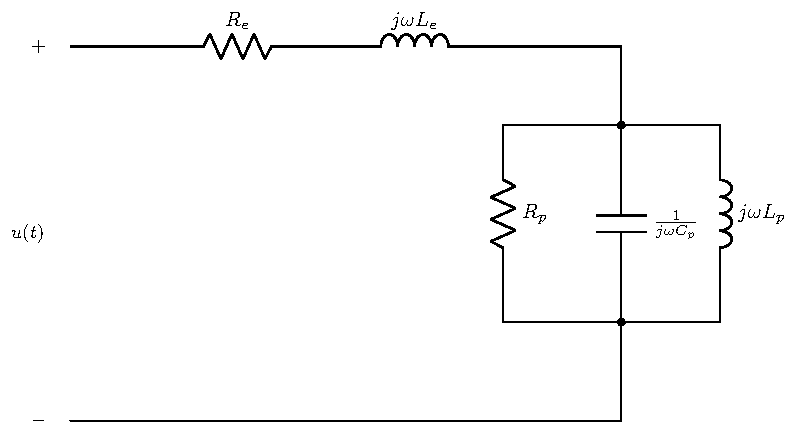
\includegraphics[width=0.5\linewidth]{TU Delft Booming Bass Project Report/figures/FilterGroup/impedance_model_phasor.pdf}
    \captionsetup{justification=raggedright, labelfont=bf}
    \caption{Equivalent model of the circuit in phasor domain.}
    \label{fig:/model_phasor}
\end{figure}

\section{Filters - Filter design}
\subsubsection{Order of the Filters}
The initial requirement is choosing the order of the filter. This will be the base of the entire filter, as it decides what type of components the filter uses. The order of the filter changes the rate at which its amplitude responds around its cut-off frequencies. The transfer function of a first-order filter will decline by 20 decibels per decade (20dB/decade), whereas a second-order filter's transfer function will decline by 40 decibels per decade (40dB/decade). 

The significance of the greater decline is that the filter will act closer to an ideal filter, which would, therefore, make it fit closer to the models made for these filters. This is because, at the cut-off frequency, the filters' amplitude response will decrease to the half-power amplitude quicker with a steeper decline in the amplitude. At and after the half-power amplitude, it can be approximated that the frequencies have a negligible impact on the speaker cone, as their power is not enough to significantly amplify the sound. Therefore, it was reasoned that a second-order filter was in the best interest of the amplifier, as it would allow the filters to be bound more to the frequencies assigned to them and have an insignificant impact outside this range. 

\subsubsection{Zobel Network}
As shown in \sfautoref{fig:/model vs measured impedance}, the impedance of the speaker increases at higher frequencies, which can lead to an increase in voltage across the loudspeaker. Consequently, this results in an increase in the difference of sound pressure produced by the speaker, as referenced in \cite{IP-manual}.

There are two potential solutions to mitigate this issue and its undesirable effect on the filters. The first is to account for the frequency-dependent impedance of the speaker in the design. The second option is to add a Zobel network parallel to the filter. A Zobel network consists of components connected in parallel with the speaker element to ensure that the combined impedance is purely resistive (In the real domain). This results in a constant impedance, simplifying the calculation process.

However, designing a Zobel network presents challenges, as it requires simulating the network to determine the optimal component values. Even once this is achieved, the limitations of available components in the lab may prevent the Zobel network from eliminating the reactance of the loudspeaker (the complex part of the impedance). It is more likely to only reduce the frequency dependence of the impedance. Based on these considerations, the group decided that implementing a Zobel network was not appropriate for this project, and therefore it was not used.

\subsubsection{Cut-off Frequency Calculations}
The cut-off frequencies are defined as the points where the transfer functions gain reaches $\sqrt{2}/2$, commonly referred to as the -3dB frequency. For low-pass filters, frequencies above this point have minimal and, thus, a negligible effect on the output. In the case of a band-pass filter, there are two cut-off frequencies; frequencies outside this range, both before the first and after the second cut-off, do not significantly affect the output. Lastly, for high-pass filters, the frequencies before the cut-off frequencies do not have a significant effect on the output.

Selecting the appropriate cut-off frequencies is crucial, as the primary goal of the project is to achieve the flattest possible acoustic response. The cut-off frequencies determine the optimal frequency ranges for each speaker, ensuring that each cone operates within its optimal range. Tweeters perform best at high frequencies (2kHz - 20kHz), bass at low frequencies (\~40Hz - 400Hz), and mid-toners in the middle range. Frequencies outside this range can either degrade the sound quality or potentially damage the speaker cone. Therefore, it is essential to carefully select these cut-off frequencies.
The optimal cut-off frequencies were determined by overlaying the acoustic responses of each speaker using Python, as shown in \sfautoref{fig: Cutoff frequencies}. By visual inspection and understanding each speaker's ideal frequency range, the cut-off frequencies were selected. The approach involved identifying the frequencies where each speaker began to show instability and where the next speaker could take over smoothly in their frequency range. This careful selection, accounting for constructive and destructive interference between sound waves, allowed for the flattest possible overall response.

The final choice for the low-pass filter's cut-off frequency was 200Hz, as it produced the flattest overall acoustic response, as seen in \sfautoref{fig: Cutoff frequencies}. For the high-pass filter, the cut-off frequency was set at 1250Hz to provide a smooth transition between the high-pass and band-pass filters. However, it is important to note that at 900Hz in \sfautoref{fig: Cutoff frequencies}, there is a noticeable dip in the mid-toner's power response. This dip affects the overall response before the cut-off frequency. Despite efforts to select the optimal cut-off frequencies, this dip remained a factor to be cautious of in the design process.
\begin{figure}[H]
    \centering
    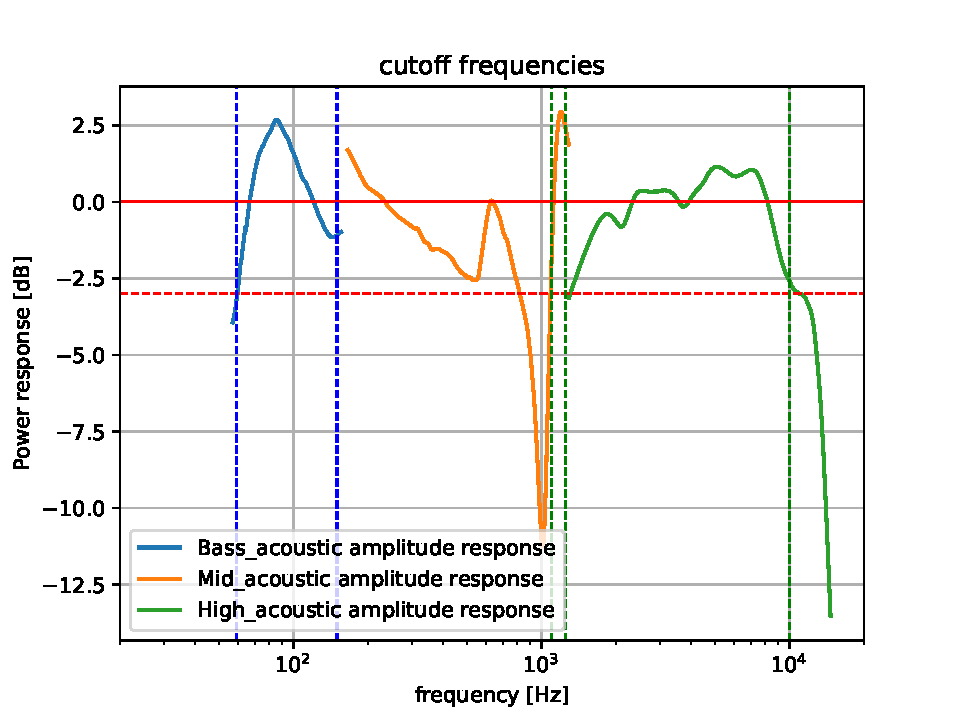
\includegraphics[width=0.65\linewidth]{TU Delft Booming Bass Project Report/figures/FilterGroup/chosenvalues.pdf}
    \captionsetup{justification=raggedright, labelfont=bf}
    \caption{Amplitude responses of the various filters plotted to aid in selecting the initial cut-off frequencies, denoted by $\omega_c$, for optimal frequency separation.}
    \label{fig: Cutoff frequencies}
\end{figure}

\subsubsection{Filters Transfer Function}
The transfer functions of the filters describe the relationship between the input voltage and the output voltage of the filter. By using \seautoref{eq:transfer_function}, a relevant transfer function can be derived for each filter, enabling the analysis of their frequency responses. This approach is invaluable in the design process, as it allows for a comprehensive examination of the filter's behavior across a wide range of frequencies. Such an analysis helps ensure that the filter performs as expected and meets the desired specifications, guiding the optimization of filter parameters.

The High-Pass Filter (HPF) is composed of components shown in \sfautoref{fig:HighPassFilter}. In this configuration, the loudspeaker impedance, denoted as $Z_l$, is modeled as a single component. By applying nodal analysis to the high-pass filter circuit in \sfautoref{fig:HighPassFilter}, the transfer function, as expressed in \seautoref{High pass filter Transfer function}, can be derived. This transfer function characterizes the relationship between the input and output voltages of the filter, facilitating the analysis of the filter's behavior across different frequencies.
\begin{flalign}
    \label{High pass filter Transfer function}
    \mathbf{H_{HPF}(\omega)} = \frac{C_HL_HZ_l\omega^2}{C_HL_HZ_l\omega^2-j\omega L_{H}-Z_l}
\end{flalign}

where $C_H$ and $L_H$ are the capacitance and inductance of the High-Pass Filter (LPF), denoted by subscript $H$, respectively.
Furthermore, the Low-Pass Filter in Fig \ref{fig:LowPassFilter} was analyzed with nodal analysis, which resulted in the transfer function in Eq \ref{Low pass filter Transfer function}
\begin{flalign}
    \label{Low pass filter Transfer function}
    \mathbf{H_{LPF}(\omega)} = \frac{-Z_l}{L_LC_LZ_l\omega^2-j\omega L_{L}-Z_l}
\end{flalign}

where $C_L$ and $L_L$ are the capacitance and inductance of the Low-Pass Filter (LPF), denoted by subscript $L$, respectively.
Moreover, the band-pass filter in Fig \ref{fig:BandPassFilter} was examined with nodal analysis, where the transfer function in Eq \ref{Band pass filter Transfer function} was found.
\begin{flalign}
    \label{Band pass filter Transfer function}
    \mathbf{H_{BPF}(\omega)} = \frac{jC_HL_HZ_l\omega^2}{-jC_HC_LL_HL_LZ_l\omega^4-C_HL_HL_L\omega^3+jZ_l\omega^2(C_HL_H+C_LL_H+C_LL_L)+(L_H+L_L)\omega-jZ_l}
\end{flalign}
\begin{figure}[H]
    \centering
    \begin{minipage}{0.29\textwidth}
        \centering
        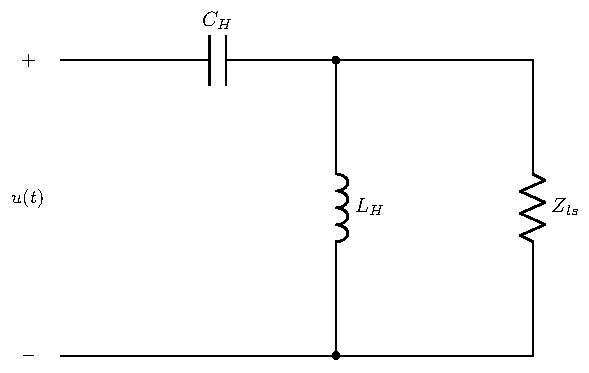
\includegraphics[width=\linewidth]{TU Delft Booming Bass Project Report/figures/FilterGroup/High pass filter schematic.pdf}
        \captionsetup{justification=centering}
        \subcaption{High-pass filter schematic.}
        \label{fig:HighPassFilter}
    \end{minipage}%
    \hfill
    \begin{minipage}{0.29\textwidth}
        \centering
        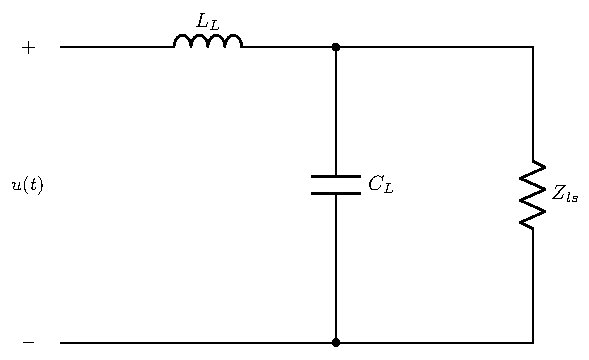
\includegraphics[width=\linewidth]{TU Delft Booming Bass Project Report/figures/FilterGroup/Low pass filter schematic.pdf}
        \captionsetup{justification=centering}
        \subcaption{Low-pass filter schematic.}
        \label{fig:LowPassFilter}
    \end{minipage}%
    \hfill
    \begin{minipage}{0.36\textwidth}
        \centering
        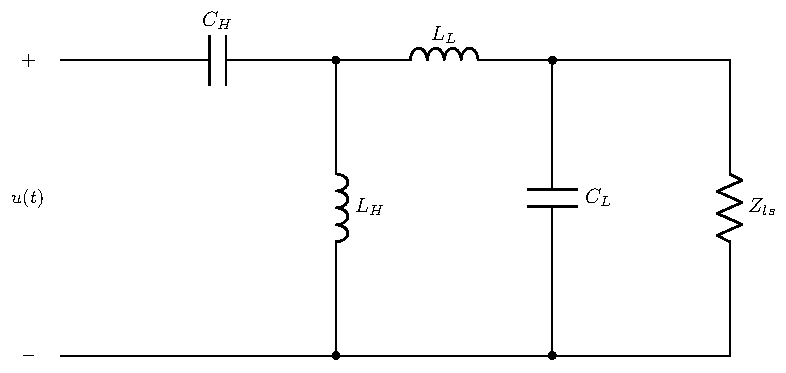
\includegraphics[width=\linewidth]{TU Delft Booming Bass Project Report/figures/FilterGroup/Band pass filter schematic.pdf}
        \captionsetup{justification=centering}
        \subcaption{Band-pass filter schematic.}
        \label{fig:BandPassFilter}
    \end{minipage}
    \captionsetup{justification=raggedright, labelfont=bf}
    \caption{Schematics of different filters used in the project. (a) High-pass filter, with components $C_H$ and $L_H$ representing the HPF capacitance and inductance. (b) A low-pass filter (LPF), where $C_L$ and $L_L$ are the LPF capacitance and inductance. (c) A band-pass filter (BPF), designed by combining the characteristics of both HPF and LPF to achieve the desired frequency separation. These schematics illustrate the design of the three filters implemented to optimize the frequency response for the sound amplifying system.}
    \label{fig:FilterSchematics}
\end{figure}



\subsubsection{Component Value Calculations}
To build the filters, the specific values of the components must be found. The values of the components change the cut-off frequencies of the filters. Eq \ref{Cutoff frequency formula} can be used to find the cut-off frequency for a second-order filter. Therefore the right components must be chosen to have the right cut-off frequencies. 

Python was used to find the values of the components that would give a cut-off frequency as close as possible to the decided frequency. As seen in appendix \ref{chapter: Code}, there was a list of available values that was iterated through. It would calculate the cut-off frequency with Eq \ref{Cutoff frequency formula} and store the difference it had with the desired cut-off frequency. This was compared to the next pair until the best pair of inductor and capacitor for both high pass and low pass filters was found. 
\begin{flalign}
    \label{Cutoff frequency formula}
    f_c = \frac{1}{2\pi\sqrt{LC}}
    \equnit{\si{Hz}}
\end{flalign}

When the component values were found, the filters were tested in LTSpice. It was then found that the components were a successful match, as the cut-off frequencies matched the desired ones closely. This allowed the filters to be built and tested in real. 
